%File: formatting-instruction.tex
\documentclass[letterpaper]{article}
\usepackage{aaai}
\usepackage{times}
\usepackage{helvet}
\usepackage{courier}
\usepackage{amsmath}
\usepackage{tikz}
\usepackage{graphicx}
\usetikzlibrary{shapes,arrows,automata}

\frenchspacing
\pdfinfo{
/Title (Unsupervised Modelling of Patient-level Disease Dynamics)
/Subject (AAAI Publications)
/Author (AAAI Press)}
\setcounter{secnumdepth}{0}
\begin{document}
% The file aaai.sty is the style file for AAAI Press
% proceedings, working notes, and technical reports.
%
\title{Unsupervised Modeling of Patient-level Disease Dynamics}
\author{S. Tamang and S. Parsons\\
Brooklyn College and The Graduate Center\\
The City University of New York (CUNY)\\
New York, NY USA\\
}
\maketitle
\begin{abstract}
To provide insight into patient-level disease dynamics from data collected at irregular time intervals, this work extends applications of semi-parametric clustering for temporal mining.  In the semi-parametric clustering framework, Markovian models provide useful parametric assumptions for modeling temporal dynamics, and a non-parametric method is used to cluster the temporal abstractions instead of operating on the original data.   Our contribution extends abstraction to continuous-time Markov models and the clustering component to the non-parametric Bayesian setting, which does not require the number of clusters to be indicated a priori.
\begin{quote}
\end{quote}
\end{abstract}

\section{Introduction}
\noindent
To provide a better understanding of dynamic changes that can occur during the course of a patient's disease trajectory, this work applies exploratory analysis methods to temporal data.  One major challenge posed by modeling patient level data is that disease related observations are typically documented only during hospital or physician visits, resulting in irregular time intervals.  Also, a patient's measurement sequence be short or can span over many years and the nature of the observation scheme (e.g., fixed, random or self-selected) can be unclear.

Rather than use the sequences of values directly, and based on recent work outlining a framework for \emph{semi-parametric clustering} of time series data (Jebara 2007), we build probabilistic models, abstractions, of these sequences using continuous-time models.  Specifically, we extends temporal abstraction to multi-state hidden Markov models, which are an instance of continuous-time hidden Markov models (CT-HMMs).

In addition to abstraction with a continuous-time model, we extend the clustering component to the non-parametric Bayesian setting, allowing for the number of clusters to be expressed as a function of the sample size.  Determining the number of clusters, $k$, is a challenge posed by many traditional clustering algorithms.

%Although there has been extensive work on the development of approaches for clustering temporal patient in more intensive sampling environments, such as an ICU, these do not easily translate to longer-term longitudinal data, where irregularly sampled over days or years is common.  Also, there is work on patient clustering is often performed on cross-sectional data, that is limited in its ability to capture dynamic patterns that are critical to understanding the manifestation and trajectory of many common diseases, or by discretizing time, forces assumptions about disease state values when data is absent.

\subsection{Application to Data Driven Wellness}
\noindent
Temporal data can provide critical contextual information to discover new knowledge relevant to health and wellness.  However, the accumulation of patient data has outpaced the generation of effective methods for temporal analysis.  Although there is extensive work on approaches for modeling patients in environments such as the ICU, these do not easily translate to long durations, such as months or years.  To this end, we demonstrate a clustering method for the exploratory analysis of longitudinal patient data that easily extends to new data sets, and in contrast to discrete time approaches, is more appropriate for modeling incomplete, irregular observation sequences that are common to patient data found in electronic health records.


\section{Temporal Representations}
Regardless of the temporal mining task, the first step of an algorithm is to transform, or abstract, the raw data into a more concise representation, preserving as much of the information contained in the original sequence as possible. The specific models we use are based on finite state continuous time Markov processes.

Markovian models are based on the underlying assumption that the future state of a system, $Q_{t+1}$, is independent of all past states, given the current state $Q_{t}$.  Hidden Markov models (HMMs) are useful for representing phenomena that care not directly observed, but for which a correlated variable can provide sufficient information to make inferences about the latent or \emph{hidden} state's value.

HMMs are defined by a triple, $\{ A, B, \pi \}$ over a set of discrete states and distinct observations.  The matrix $A$ represents the state transitions, or the probability of moving from the current state, $q_{i}$, to the next state, $q_{i+1}$. The model parameter $B$ indicates the probability of an observation value for each $q\in Q$.

Although discrete-time models are suitable in many cases, there are two key limitations that have been noted (Saria 2007) and are directly relevant to the type of data typically found in provider databases.  First, if the underlying health related phenomena that is being modeled progresses in individuals at different rates, the smallest granularity must be used to express time steps for the entire system.  Second, when data is unavailable, intervening time slices must still be represented.

\subsection{Multi-state Markov Models}
By default, all traditional HMMs, and dynamic Bayesian networks more generally, make discrete-time assumptions. A main distinguishing characteristic between DT and CT HMMs is that in the discrete-time case, the Markov process stays in a state $i$ for a time distributed according to $F_{i}(t)$ and in the continuous-time case the holding time is \emph{exponentially} distributed according to $F_{i}(t) = e^{q_{i}t}$ where $q_{i}$ is the intensity of the transitions, or the tendency to change state.

For a process variable $X$ with a domain of of ${x_1,x_2,...,x_n}$ where $n$ corresponds with the number of states, the intuition is that the intensity, $q_{i}$, no longer corresponds with the transition probability that is constant for the length of a time slice, but rather an `instantaneous probability' of leaving state $x_i$ and the intensity of $q_{i,j}$ gives the `instantaneous probability' of transitioning from $x_i$ to $x_j$.

\begin{figure}[h!]
\begin{center}
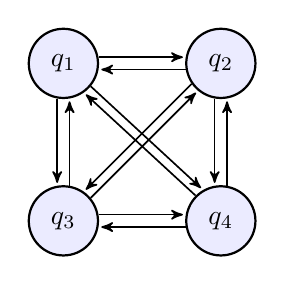
\begin{tikzpicture}[->,>=stealth',shorten >=1pt,auto,node distance=2cm,semithick]
\tikzstyle{every state}=[fill=blue!8,draw=black,thick,text=black,scale=1]


\node[state]         (A)              {$q_{1}$};
\node[state]         (B) [right of=A] {$q_{2}$};
\node[state]         (C) [below of=A] {$q_{3}$};
\node[state]         (D) [below of=B] {$q_{4}$};


\path (A.10) edge  [right] node[right] {} (B.170);
\path (A.260) edge  [right] node[below] {} (C.100);
\path (A.320) edge  [right] node[below] {} (D.120);
\path (B.190) edge  [right] node[left] {} (A.350);
\path (B.215) edge  [right] node[below] {} (C.55);
\path (B.260) edge  [right] node[below] {} (D.100);
\path (C.40) edge  [right] node[above] {} (B.230);
\path (C.80) edge  [right] node[above] {} (A.280);
\path (C.10) edge  [right] node[right] {} (D.170);
\path (D.190) edge  [right] node[left] {} (C.350);
\path (D.135) edge  [right] node[above] {} (A.305);
\path (D.80) edge  [right] node[above] {} (B.280);
\end{tikzpicture}
\[
Q_X =
  \begin{bmatrix}
    q_{1,1} & q_{1,2} & q_{1,3} & q_{1,4}\\
    q_{2,1} & q_{2,2} & q_{2,3} & q_{2,4}\\
    q_{3,1} & q_{3,2} & q_{3,3} & q_{3,4}\\
    q_{4,1} & q_{4,2} & q_{4,3} & q_{4,4}\\
  \end{bmatrix}
\]
\end{center}
\caption{Multi-state Markov Model}
\label{fig:msm}
\end{figure}

The specific instance of CT-HMMs we use for temporal abstraction are hidden multi-state Markov models (MSMs).  A 4 state MSM is shown in Figure \ref{fig:msm}, with the intensity matrix $Q$ that represents the instantaneous behavior of the process $X$.  The states are ordered progressively to reflect stages in a disease trajectory.   MSMs are not well known outside epidemiology and biostatistics, where they have applied for chronic disease modeling at the population level and have hidden and semi-Markovian extensions (Jackson 2011).

\noindent
\section{Non-parametric Bayesian Clustering}
\noindent
A main challenge posed by many traditional clustering algorithms is selecting the number of components.  Using a Dirichlet process (DP) Gaussian mixture model for non-parametric Bayesian clustering, we group patients by disease dynamics using the abstractions of their raw measurement sequences.

The Dirichlet process is a measure on measures that is characterized by two parameters: a base distribution $G_0$, from which samples are drawn, and a positive scaling parameter $\alpha$, which is more intuitively described as a `splitting' criteria and is associated with the probability of forming a new cluster.  For a sample, $G$, drawn from the base distribution $G_0$, if $G \sim DP(G_0,\alpha)$ then for any set of partitions $A_1 \cup A_2 \cup ... A_k$ of $A$:
$$(G(A_1),...,G(A_k)) \sim Dir(\alpha G_0(A_1),...,\alpha G_0(A_k))$$

In the the Dirichlet process mixture model, the DP is used as nonparametric prior in a hierarchical Bayesian model, where $G$ can be partitioned according to the value of the parameters.  To compute the model likelihoods and posterior distribution of the clusters we used a mean variational inference for the infinite Gaussian mixture model instead of Gibbs sampling using (Pedregosa 2011).

\section{Data and Methods}
 We apply our clustering approach to two de-identified data sets, which reflect patients with variable observation durations, measurement granularities, and levels of incompleteness associated with their record.  The first consists of a standard lab test for hepatitis, \emph{platelet counts}.  The gold standard for diagnosing the final stage of chronic liver disease is by biopsy, but the cost and invasive has created a need for alternatives.

Our second data set is from a large urban hospital, and indicates the \emph{presence or absence of glucose tests} for patients.  Typically, a single incident of a lab test may corresponds with an one-day visit or stay, or one that does not require ongoing glucose monitoring.  However, a series of contiguous testing patterns likely correspond to a patient with diabetes that is being actively monitored.

We estimated $n$, the number of states for the models using a non-parametric Bayesian density estimator.  Since the number of states and the continuous nature of the model should not be too large, the upper-bound on the number for density estimation was set to a maximum of five.  Platelet count values were used directly for estimating the number of states.  The glucose testing data was processed before state estimation.  Creating a new vector, we set the observation value to the number of days contiguous tests were ordered.  For example, and measurement sequence of $[1,0,0,0,1,1,1,1]$ would consist of two observations, 1 and 4.

Initial values for the each patients intensity matrix were obtained by using a naive estimation provided by counting the total number of transition pairs for the entire population, and estimating their probability of occurrence. Although not all patients were able to have model parameters output by the abstraction method, initial population level estimates allowed more observations to converge using the parameter estimation methods than the same naive initialization assumption at the patient level.

Using a 4-state multi-state Markov model, each patient's parameters are calculated using likelihood estimations based on the time and values in their observation sequences.  The parameter, or abstraction, used as input to clustering is the matrix $Q$, representing the instantaneous behavior of the process $X$, as an $n$x$n$ matrix.
\noindent
\section{Results}
\noindent
To validate the results of clustering platelet count values for the hepatitis data set, we used grading and staging data from liver biopsies. Figure~\ref{biopsy} show the result from the clustering with the highest highest purity (0.61\%) and obtained using continuous-time HMM abstraction paired with non-parametric Bayesian clustering.  Cluster purity obtained using spectral clustering, was notably lower, reporting a high of $0.40$.  Cluster membership is visualized in relation to highest biopsy grading, and reported by percent of the total for each grade ($n=468$).  A grading of four indicates cirrhosis of the liver or advance scarring. In addition to grading, biopsy activity is commonly used to stage liver disease and visualized in Figure 2. using the fill variation for each pie.

\begin{figure}[h]
\centering
\includegraphics[width=85mm]{fig/hep_2.jpg}
\caption{Hepatitis Clusters by Biopsy Staging and Activity}
\label{biopsy}
\end{figure}

External data for validating our glucose data set clustering was not available and intrinsic measures based on cluster silhouettes were used to assess cluster quality.  The results of CT-HMM abstraction paired with non-parametric Batesian clustering paired is reported in terms of average silhouette is shown in~\ref{table:sil}.  Spectral clustering was also paired with CT-HMMs.  Although the average silhouette value was overall lower (0.10), one large cluster had a average silhouette higher that that on the max for non-parametric Bayesian clustering.

\begin{table}[h]
\caption{Cluster Silhouettes}
\centering
\begin{tabular}{|l|c|c|}
  \hline
  % after \\: \hline or \cline{col1-col2} \cline{col3-col4} ...
   Cluster& Members & Average Silhouette  \\
   \hline
  $C_1$ & 153 & -0.04956 \\
  $C_2$ & 269 & 0.9416  \\
  $C_3$ & 132 & 0.1151  \\
  $C_4$ & 114 & -0.3712 \\
  $C_5$ & 337 & -0.5460 \\
  \hline
\end{tabular}
\label{table:sil} % is used to refer this table in the text
\end{table}

Compared with discrete-time HMM abstraction for the same data set, in previous work (Tamang 2011) we reported over 80 percent of patients with a good (0.60 or above) silhouettes value.  In comparison, continuous-time HMM abstraction report just over half of patients with a good silhouette value (54 percent).

\section{Conclusions}
\noindent

We demonstrate a new method to model patient disease dynamics with two key features.  First, we use continuous-time (CT) HMM abstraction, which avoids some of the limitations of discrete-time approaches when a dynamic process evolves at different time granulations, and when observations are irregularly sampled and missing not at random.  Second, non-parametric Bayesian clustering methods avoid the problem of identifying the number of clusters a priori, inferring the appropriate number of mixture component as a function of the sample size.

Specifically, we apply hidden multi-State models, an instance of continuous-time HMM models used by biostatistican for disease modeling.  Although we were unable to match the intrinsic clustering quality achieved in previous work using discrete-time HMMs abstraction with glucose test data, performance was comparable.  However, on a hepatitis data we externally validate their effectiveness.  We also assess the performance of pairing temporal abstraction with a non-parametric Bayesian clustering.  It conveniently eliminates the need to estimate $k$, and  performed better that spectral clustering on the hepatitis data set.

 Our continued work will focus on more rigorous, and alternative methods for cluster evaluation. Silhouette values are limited in their ability to assess quality and there may be more suitable, or additional methods to evaluate clusters.  Also, in terms of external validation for our hepatitis data set, our clusters are not categorical, but rather ordinal and accounting for the relations between clusters may also provide additional insights into the performance our techniques.

\subsection{References}
%Oprevious work (Tamang 2011) compared DT-HMMs relative to aggregate time series statistics. Our results demonstrated the benefit of pairing DT-HMM abstraction and spectral methods for clustering temporal data.  Improved cluster quality was consistently achieved using DT-HMMs, suggesting that Markov models provide useful parametric assumptions for modeling temporal data.  Also, spectral clustering consistently reported better performance, suggesting that more agnostic assumptions about the cluster shape benefits overall performance.

\smallskip \noindent Jackson, C. 2011. Multi-State Models for Panel Data: The msm Package for R. \textit{Journal of Statistical Software} 38(8): 1--29.

\smallskip \noindent Saria, S; Nodelman, U.; and Koller, D. 2007. Reasoning at the Right Time Granularity. \textit{Proceedings of the Twenty-third Conference on Uncertainty in AI}, 421--430.
	
\smallskip \noindent Jebara, T.; Song, Y.; and Thadani, K. 2007. Spectral clustering and embedding with hidden Markov models. \textit{In Proceedings of the 18th European Conference on Machine Learning}, 164-175.

\smallskip \noindent Tamang, S.; and Parsons, S. 2011. Using semi-parametric clustering applied to electronic health record time series data. \textit{In Proceedings of the 17th ACM SIGKDD: Workshop on Data Mining for Medicine and Healthcare}, 72--75.

\smallskip \noindent Pedregosa, F.; Varoquaux, G.;Gramfort, A.; Michel, V.; Thirion, B.; Grisel, O.; Blondel, M.; Prettenhofer, P.; Weiss, R.; Dubourg, V.; Vanderplas, J.; Passos, A.; Cournapeau, D.; Brucher, M.; Perrot, M. and Duchesnay, E. 2011. Scikit-learn: Machine Learning in Python. \textit{Journal of Machine Learning Research}, 12: 2825--2830.
\end{document} 